\documentclass[letterpaper, 10 pt, conference]{ieeeconf}  % Comment this line out if you need a4paper

%\documentclass[a4paper, 10pt, conference]{ieeeconf}      % Use this line for a4 paper

\IEEEoverridecommandlockouts                              % This command is only needed if 
                                                          % you want to use the \thanks command

\overrideIEEEmargins                                      % Needed to meet printer requirements.

%\renewcommand{\baselinestretch}{2}
\pdfminorversion=4
\usepackage{tikz}
\usetikzlibrary{shapes,arrows}



% See the \addtolength command later in the file to balance the column lengths
% on the last page of the document
\newtheorem{theorem}{Theorem}[section]
\newtheorem{corollary}{Corollary}[theorem]
\newtheorem{lemma}[theorem]{Lemma}
\usepackage{amsmath} 
\usepackage{amssymb} 


\usepackage{ltl} 

\usepackage{algorithm2e}

\usepackage{color}
\usepackage{subfig}
\usepackage{tikz}
\usetikzlibrary{arrows,fit,shapes,automata}
\usetikzlibrary{positioning,fit,calc,shapes}
\usetikzlibrary{decorations.fractals}
\usetikzlibrary{decorations.markings}

\newcommand{\Rayna}[1]{{\textcolor{magenta}{ \textbf{Rayna:} #1 $\spadesuit$ }}}
\newcommand{\Suda}[1]{{\textcolor{blue}{ \textbf{Suda:} #1 $\spadesuit$ }}}
\newcommand{\Ufuk}[1]{{\textcolor{red}{ \textbf{Ufuk:} #1 $\spadesuit$ }}}
\newcommand{\todo}[1]{{\textcolor{red}{TODO:} #1}}

% Local macros
\providecommand{\st}{\mathrel{\mid}}
\newcommand{\defeq}{:=}
\newcommand{\pow}[1]{2^{#1}}
\newcommand{\supp}{\mathsf{supp}}
\newcommand{\reach}{\mathsf{Reach}}
\newcommand{\dist}[1]{\mathcal{D}(#1)}
\newcommand{\ie}{\textit{i.e.}\xspace}
\newcommand{\eg}{\textit{e.g.}\xspace}
\newcommand{\myparagraph}[1]{\par\smallskip\noindent\textbf{#1.}}
\newcommand{\prob}{\mathcal{P}}
\newcommand{\polreachp}[4]{\prob_{#1}^{#2,#3}[\mathrm{Reach}(#4)]}
\newcommand{\maxreachp}[3]{\mathrm{Val}_{#1}^{#2}(#3)}


\newtheorem{example}{Example}

\newcommand{\init}{\mathsf{init}}
\newcommand{\belief}{\mathsf{belief}}
\newcommand{\abstr}{\mathsf{abstract}}
\newcommand{\vis}{\mathit{vis}}
\newcommand{\succs}{\mathit{succ}}
\newcommand{\beliefs}{\mathcal{P}(L_t)}

\newcommand{\Surveillance}{\mathsf{Surveillance}}
\newcommand{\beliefF}{\mathit{belief}}

\newcommand{\states}{S}
\newcommand{\trans}{T}
\newcommand{\part}{\mathcal{Q}}

\newcommand{\post}{\mathit{post}}

\newcommand{\outcome}{\mathit{outcome}}
\newcommand{\counterex}{\mathcal{C}}

\newcommand{\bools}{\mathbb{B}}
\newcommand{\true}{\mathit{true}}
\newcommand{\false}{\mathit{false}}
\newcommand{\nats}{\mathbb{N}}

\newcommand{\SP}{\mathcal{SP}}
\newcommand{\AP}{\mathcal{AP}}
\DeclareMathOperator*{\argmin}{arg\,min}




   
\def\fat#1{#1}

\title{Minimal-Information Control of MDPs with Temporal Logic Constraints
}

\author{Suda Bharadwaj$^{1}$ \and Takashi Tanaka$^{1}$ \and Ufuk Topcu$^{1}$% <-this % stops a space
%\thanks{*This work was not supported by any organization}% <-this % stops a space
\thanks{$^{1}$ Suda Bharadwaj, Takashi Tanaka, and Ufuk Topcu are with the Department of Aerospace Engineering and Engineering Mechanics at the University of Texas at Austin. E-mail: \{sudab, ttanaka, utopcu\}@utexas.edu}%
%\thanks{$^{2}$Bernard D. Researcheris with the Department of Electrical Engineering, Wright State University, Dayton, OH 45435, USA {\tt\small b.d.researcher@ieee.org}}%
}


\tikzstyle{block} = [draw, fill=blue!20, rectangle, 
    minimum height=3em, minimum width=6em]
\tikzstyle{sblock} = [draw, fill=blue!20, rectangle, 
    minimum height=3em, minimum width=3em]
\tikzstyle{sum} = [draw, fill=blue!20, circle, node distance=1.2cm]
\tikzstyle{input} = [coordinate]
\tikzstyle{output} = [coordinate]
\tikzstyle{pinstyle} = [pin edge={to-,thin,black}]



\begin{document}

\maketitle
\thispagestyle{empty}
\pagestyle{empty}

%%%%%%%%%%%%%%%%%%%%%%%%%%%%%%%%%%%%%%%%%%%%%%%%%%%%%%%%%%%%%%%%%%%%%%%%%%%%%%%%

\begin{abstract}
We consider Markov decision processes (MDPs) in which the information cost quantified by transfer entropy is added to an objective specified as a co-safe linear temporal logic (LTL) formula. We assume some of the state variables are expensive to measure, and the information cost is given by the transfer entropy from the specified state variables to the control action. We then find the policy that acts to minimize the weighted sum of the information cost and the cost of failing to satisfy the specification. We provide a method to synthesize a policy that minimizes the weighted sum of the information cost and the probability of failure to satisfy the LTL specification. We solve the problem by deriving sufficient conditions for optimality, and compute the optimal policy using a modified Arimoto-Blahut algorithm. Finally, we present a numerical experiment involving navigation and path planning and demonstrate the effect of adding information cost to certain state variables.
\end{abstract}

%%%%%%%%%%%%%%%%%%%%%%%%%%%%%%%%%%%%%%%%%%%%%%%%%%%%%%%%%%%%%%%%%%%%%%%%%%%%%%%%

\section{Introduction}
Autonomous systems are expected to complete increasingly more complex missions in dynamic and uncertain environments. In space applications, in particular, these systems are in addition  fettered by communication or sensing restrictions. For instance, in the upcoming  Mars 2020 rover mission,  a Mars rover is tasked to safely explore an uncertain environment  and coordinate with a scouting helicopter~\cite{landau2015helicopter}. Missions of such sophisticated nature will necessitate on-board autonomy \cite{francis2017advanced,estlin2007increased}. Nonetheless, tight sensing constraints, due to the power consumption of on-board sensors and transmitters, and  bandwidth limitation on data sent from the Earth and orbiting satellites \cite{sherwood2014,Backes1999} further complicates the navigation task. In these cases, it is necessary  for autonomous agents to make decisions with \emph{limited information} and  complete their mission specification above an acceptable threshold. %In some situations, there is not enough time to transmit all sensor data before a control decision can be made. For example, in distributed control of UAVs that may need to react quickly to changes in the environment \cite{Baillieul07}. 

Markov decision processes (MDPs) are one of the most widely studied models for decision-making under uncertainty in the fields of artificial intelligence, robotics, and optimal control \cite{Papadimitriou87}. We model the interaction between the uncertain environment and the autonomous agent using a Markov decision process~(MDP) with an additional \emph{transfer entropy} cost that we refer to as a TEMDP~\cite{takashi17}.   We use the additional transfer entropy cost~\cite{schreiber2000} to quantify the directional information flow  from the state of an MDP (representing the uncertain environment or the location of the autonomous agent) to the control policy. Intuitively, minimizing the transfer entropy promotes policies that rely less on knowledge of the current state of the system. In communication theory, a related quantity called \emph{directed information} has been used to measure channel capacities in feedback systems \cite{massey1990causality,tatikonda2009capacity} as well as a proxy for feedback data rate to controllers \cite{silva2011achievable}. 

%However, transfer entropy is often used for studying causality in fields including statistical thermodynamics \cite{parrondo2015thermodynamics}, neuroscience \cite{vicente2011transfer}, and biology \cite{tung2007inferring}. Transfer entropy has also been previously used with policy synthesis in MDPs in \cite{takashi17}, though without temporal logic specifications. 

There has been a lot of work on quantifying information requirements for low-level control requirements, such as stability~\cite{Nair07}. However, quantifying information requirements for high level decision making scenarios that we are interested in are not as widely studied. This is analogous to model reduction techniques for MDPs under temporal logic constraints studied in \cite{Bharadwaj17,brazdil2014verification,ciesinski2008reduction}, where states and actions that are completely irrelevant to the mission are removed.~\cite{Tishby2011} examines directed information in MDPs to quantify information. Policies are penalized if they vary too much from a completely uninformed starting point, e.g, take any action with equal probability. We are, on the other hand, interested in studying the causality of information from the state to the controller, i.e, we seek to penalize sending information that is not relevant for the decision-making process. Hence, transfer entropy is a better information-theoretic metric in our setting. 

%Our work can be seen as a generalization of \cite{takashi17}, where the transfer entropy is also used, but the authors do not allow the possibility of penalizing certain sensors over others. This is crucial in settings where different sensors can have varying energy costs and is hence necessary to budget the use of certain sensors to conserve energy. Furthermore, in distributed control of multiple agents, it is sensible to reduce the reliance of information transmitted from other agents compared to information from on-board sensors due to bandwidth restrictions in transmission.
%



%
%Hence, understanding the effects of limiting the information flow to the policy synthesizer is key towards pushing the use of MDPs in information-constrained applications. 

% like Mars rovers. This will allow us to take exploit the existing well studied techniques in controlling MDPs to use in communication and sensing constrained situations. 

%Defining sophisticated mission objectives in MDPs requires specifying complex reward functions in order to synthesize a control policy \cite{puterman2014}. 
Furthermore, we consider high-level mission specifications that are defined in terms of temporal logic. Temporal logic has been used as a formal way to allow the user to relatively intuitively specify high-level specifications such as infinitely often patrolling a region or moving to a certain region without collisions. %Linear temporal logic (LTL) in particular has been popular for use in optimal control \cite{Svoreňová13,Fu15} as 
Several tools exist to synthesize policies in MDPs with probabilistic temporal logic specifications~\cite{Svoreňová13,Fu15}. We study the effect of information restriction on satisfying temporal logic objectives in TEMDPs. 

 %It is known that deriving controllers for rich temporal logic specifications reduces to solving a reachability problem on an MDP. 
%Related work involving planning under sensing constraints with temporal logic specifications is in cases where the knowledge of the entire state is \emph{unavailable}, \ie, only part of the state can be observed and usually modeled as POMDPs whereas we look at scenarios where full state information is available, but with restricted access. Or scenarios where the information is known, but only a limited amount can be transmitted to the controller. Specifically, we study the effect of information restriction on satisfying temporal logic objectives in MDPs.

%In order to study the effects of restricted information flow, we need to be able to quantify it.

\paragraph*{\textbf{Contributions.}} Our contributions are as follows:\\
(1) We develop a novel framework to formally connect information-theoretic techniques for policy synthesis in MDPs with techniques from formal methods and probabilistic model checking. Specifically, we include a transfer entropy cost on state variables that are 'expensive to observe', which is  minimized along with the probability of failure of satisfying a co-safe linear temporal logic formula. \\
(2) In contrast to standard MDP policy computation under temporal logic specifications, the additional information cost leads to randomized optimal policies \cite{tanaka2017lqg,Todorov09,takashi17} necessitating policy search in an infinite state space. To solve this efficiently, we derive a sufficient optimality condition in the form of coupled non-linear equations. We solve this using a modified version of a forward-backward iterative algorithm from~\cite{Blahut72}.\\
(3) While the proposed method builds on earlier results in \cite{takashi17}, we generalize the setting to penalize subsets of state variables and incorporate temporal logic constraints. 

\subsection{Case Study}\label{sec:casestudy}
We demonstrate the use of information-constrained control of MDPs under temporal logic specifications in a scenario based on the upcoming Mars 2020 mission~\cite{landau2015helicopter}. 

Mars rovers operate in mostly unknown environments. Limited a priori knowledge of the terrain and possible obstacles can be provided from satellite imagery. This information, however, is often not enough for decision-making as was evidenced by the Curiosity rover which suffered punctures due to the unexpected presence of jagged, immobile, rocks embedded in the terrain. Proposed methods to reduce damage such as driving the rover backwards requires heavy human intervention and planning. For autonomous decision-making to be viable, information on local terrain characteristics is needed for planning so a human does not need to manually avoid obstacles. For the Mars 2020 mission, a helicopter has been proposed to act as a scout \cite{landau2015helicopter} to assist with planning. Figure \ref{fig:mars2020} shows an artists' rendering of the helicopter flying ahead to scout. The helicopter can then transmit information of the terrain back to the rover which is used for path planning.

\begin{figure}
\centering
\includegraphics[scale=0.18]{mars2020.jpg}
\caption{Artist's rendering of the proposed helicopter to scout for the Mars rover. The helicopter can fly ahead and send information back to the rover about the presence of any obstacles. \cite{landau2015helicopter}.}\label{fig:mars2020}
\end{figure}

We model a scenario where the rover is tasked with collecting samples from a specific region. The environment is modeled as an MDP as motion can be stochastic, i.e, slippage can occur. The mission is specified in LTL as it allows us to easily and formally state high level tasks for the rover, and the decision-making goal is to \emph{maximize} the probability of satisfying the mission specification. The helicopter can send terrain information (such as locations of any small rocks) to the rover to assist in path planning but transmitting information costs power. We provide a method that allows the planner to maximize the probability of completing the mission while also penalizing information transfer. This means the rover must plan to satisfy the mission specification while relying on as little information from the helicopter as possible. The specifics of the experiment is described in section $\ref{sec:exp}$.
%Finally, we present a path planning example in grid worlds with moving and static obstacles and qualitatively analyze the impact of the information cost on relevant state variables.

% Control systems using multiple distributed sensors and/or processors has become increasingly popular in recent times \cite{Baillieul07}. In such scenarios, understanding communication restrictions and delays is imperative for real world applications. Indeed, a panel on future directions in control had identified control under communication restrictions to be an important future direction \cite{Murray03}.

% Accounting for cost of information is crucial in many decision-making scenarios. For example, a planetary rover may need to communicate with a ground station or orbiting satellite in order to complete its mission \cite{Backes1999}. However, there are often tight bandwidth constraints so it is necessary to only transmit the minimal amount of information possible to achieve the required performance \cite{sherwood2014}. Another example is coordinating autonomous agents in a hostile environment. In these cases it can be desirable to restrict communication to avoid detection, as well as to save power. Often, there is not enough time to transmit all sensor data before a control decision can be made such as in distributed control of UAVs that may need to react quickly to changes in the environment \cite{Baillieul07}. In these situations it is necessary to send the minimal information possible while still guaranteeing a certain amount of performance.

% Specifically, we want to synthesize a control policy in a Markov decision process (MDP) that minimizes the information reliance from the state but still performs above a minimum prescribed performance threshold. MDPs are one of the most widely studied tools for decision making under uncertainty in the fields of artificial intelligence, and robotics \cite{Papadimitriou87,Bharadwaj17} for optimal control and motion planning \cite{Ragi13,Burlet04}, so having a better understanding of information flow to controllers is key to pushing our understanding of communication restricted control. 

% We use \emph{transfer entropy} \cite{schreiber2000} to quantify the directional information flow between two random processes. Intuitively minimizing the transfer entropy promotes policies that rely less on the current state of the system. In communication theory, a related quantity called \emph{directed information} has been used to measure channel capacities in feedback systems \cite{massey1990causality,tatikonda2009capacity} as well as in studying feedback data rate to controllers \cite{silva2011achievable}. However, transfer entropy is often used when causality is being studied, usually in fields like statistical thermodynamics \cite{parrondo2015thermodynamics}, neuroscience \cite{vicente2011transfer}, and biology \cite{tung2007inferring}. Transfer entropy has also been previously used with policy synthesis in MDPs in \cite{takashi17}. 

% Defining elaborate control objectives in MDPs have been considered in \cite{puterman2014}. However, this requires specifying complex reward functions in order to synthesize a control policy. To this end, temporal logic has been used as a formal way to allow the user to more intuitively specify high level specifications. Linear temporal logic (LTL) in particular has been popular for use in optimal control \cite{Svoreňová13,Fu15} as it is widely studied and several tools exist to synthesize provably correct policies in MDPs. It is known that maximizing the probability of satisfying LTL objectives in an MDP reduces to a reachability objective ~\cite{BaierKatoen08}. 

% The focus of this paper is to minimize the transfer entropy cost from state variables in an MDP that are deemed expensive to measure or transmit to the controller whilst maintaining a minimum probability of satisfying a mission objective specified in LTL.

% The focus of this paper is situations where the state is composed of multiple state variables measured by different sensors. This is often the case in applications such as planetary rovers where different sensors can have varying energy costs and is hence crucial to budget the use of certain sensors to conserve energy. This problem can be seen as analogous to the centralized multi-agent problem, as we only want to penalize knowledge of states from other agents but not our own. It can also be seen as simply penalizing the use of certain sensors over others.

% \paragraph*{\textbf{Related work}}
% This work builds on \cite{Takashi17} where transfer entropy is also used to quantify the rate of information flow from state to the control action. However, the authors do not consider situations where the state is composed of multiple state variables measured by different sensors, not all of which are remote or expensive to measure. This is often the case in applications such as planetary rovers where different sensors can have varying energy costs and is hence crucial to budget the use of certain sensors to conserve energy. This problem can be also seen as analogous to the centralized multi-agent problem where we only want to penalize knowledge of states from other agents but not our own to limit communication between agents. 

% Early work in \textit{minimal attention} controllers was done in \cite{Brockett97} and \cite{Brockett03} where the authors implement control actions that do not require much 'monitoring'. To do this an \textit{attention} cost is used that penalizes varying control away from a constant input. \cite{Chatterjee2013} provides algorithms in a 2-player game formulation with $\omega$-regular objectives to minimize communication bandwidth requirements between processors. This was %done by treating the game as an imperfect information game with additional \textit{attention} costs and was
% shown to be EXPTIME-complete making this solution computationally infeasible in many cases. Furthermore, the cost used is once again applied to changing control action and not directly to the underlying flow of information to the controller. In our case, we do not penalize changing control action, only the access to information and this does not penalize non-trivial control laws based on limited information from the state.

% There is also related work done in the fields of optimal active sensor placement and control. ~\cite{Hoffmann10,krause2006near} use mutual information to determine the optimal time or position to sense. This is the inverse problem studied to that posed in this paper as the authors are trying to \textit{maximize} an information-theoretic term (mutual information) so the most amount of information can be obtained with minimal sensor action. This is also case in ~\cite{Naiss13} where the authors maximize directed information. Other related work such as \cite{Tishby2011} uses a Kullback-Leibler cost (as opposed to transfer entropy) that quantifies the difference in the probability distributions of controlled trajectories compared to an uncontrolled.

% \paragraph*{\textbf{Contributions}}
% We provide a formal way to connect information theoretic techniques to compute a policy in a finite state MDP that minimizes the information flow (quantified by transfer entropy) to the controller with techniques from formal methods and probabilistic model checking by including linear temporal logic constraints. Hence, our contribution generalizes existing work and also allows for more complex objectives to be achieved. As far as we are aware there is no current work that minimizes the information-theoretic cost under temporal logic constraints. As a side note, we remark that the generalized formulation proposed in this paper is needed in order to make use of the formalism of linear temporal logic.

% In contrast to standard MDP policy computation under LTL constraints, information constrained MDPs often require randomized optimal strategies \cite{tanaka2017lqg,Todorov09} and in our case we will require a policy search under an infinite state space. To this end, we exploit the structure present in the problem to derive a sufficient condition to satisfy in the form of a coupled set of nonlinear equations. We then propose a numeric forward-backward algorithm similar to that proposed in ~\cite{Blahut72} to iteratively solve these nonlinear equations. We also present path planning experiments on grid worlds using moving and static obstacles and qualitatively analyze the impact of the information cost on relevant state variables.

% Additionally, in the application of networked control systems, we provide a physical interpretation of the transfer entropy cost problem formulation. We prove that it is in fact the lower bound on the data rate of the penalized state variables that must be transmitted in order to achieve a minimal threshold of performance.

% % The contributions of this work includes:
% % \begin{itemize}
% % \item Minimizing information flow (transfer entropy) to the controller from a user specified set of state variables under linear temporal logic constraints.
% % \item Using an Arimoto-Blahut algorithm to numerically solve the optimality equations to obtain the control policy.
% % \item In the application of networked control systems, we prove that the transfer entropy cost problem formulation is in fact the lower bound on the data rate from the part of the state space that is penalized under information cost that must be transmitted in order to achieve a minimal threshold of performance.
% % \item We provide path planning experiments on grid worlds using moving obstacles and qualitatively analyse the impact of the information cost on relevant state variables.
% % \end{itemize} 
% \paragraph*{\textbf{Structure}}
% The rest of this paper will be structured as follows. In section II, we present our definitions and other notation used in this paper. We then present the formal problem statement in section III. In section IV, we derive the optimality conditions and present the numeric algorithm to compute the optimal policy in section V. In Section V we study the practical meaning of the transfer entropy cost to networked control problems, We provide experiments to analyze the impact of the information cost in section VI and analyze its impact on path planning experiments on grid worlds. Finally, we conclude in Section VII and provide future direction.
% % We want to penalize the cost of information from a \emph{subset} of the state space. Second, we will extend this to synthesize joint controllers for multiple agents in a centralized fashion. Finally, we investigate the structure and will solve for controllers in a decentralized fashion by breaking up the centralized optimization problem.

% %The following notation will be used in this paper. The sequence $\left(x_1,x_{2}...x_t \right)$ is denoted $x^t$ and the subsequence $\left(x_k,x_{k+1}...x_l \)$ is denoted by $x_{l}^{k}$. 

%%%%%%%%%%%%%%%%%%%%%%%%%%%%%%%%%%%%%%%%%%%%%%%%%%%%%%%%%%%%%%%%%%%%%%%%%%%%%%%%

\section{Preliminaries}
The sequence $(x_0,x_{1}...x_t)$ is denoted $x^t$ and the subsequence $x_l,x_{k+1}...x_k$ is denoted by $x_{l}^{k}$. We use upper-case letters to denote random variables and lower-case letters for the realizations of the corresponding random variable. \\
We denote by $\dist{\mathcal{X}}$ the set of all probability distributions on a finite
set $\mathcal{X}$, \ie all functions $f: \mathcal{X} \to [0,1]$ such that $\sum_{x\in \mathcal{X}}f(x)=1$. Finally, for a set $\mathcal{S}$, we define $2^\mathcal{S}$ as the set of all subsets of $\mathcal{S}$ and $S^{\omega}$ as the set of all infinite sequences of elements in $\mathcal{S}$
%\subsection{Markov decision processes}
% \paragraph{Markov decision processes}
% 	An \emph{MDP} is a tuple $M=(\mathcal{X},\mathcal{U},p)$ where $\mathcal{X}$ is a
% 	finite set of \emph{states},
% 	$\mathcal{U}$ is a finite alphabet of \emph{actions},
% 	$p: S\times\mathcal{U} \to \mathcal{D}({\mathcal{X}})$ is a (partial) \emph{probabilistic
% 	transition function} that assigns to a state $x\in \mathcal{X}$ and an action $u \in
% 	\mathcal{U}$ a probability distribution over the successor states. We
% 	abbreviate $p(x_{t},u)(x_{t+1})$ by $p(x_{t+1}|x_t,u_t)$.
\paragraph*{Labeled Markov decision process (MDP)} Consider a set $\AP$ of \emph{atomic propositions} which can be used, for example, to mark a state as being a ``faulty configuration'' (reaching it is, thus, undesirable), for example an obstacle. A \emph{labeled MDP} is an MDP whose states are labeled with atomic propositions. More formally, it is a tuple $M=(\mathcal{X},\mathcal{U},p,\AP,L)$ where 
\begin{itemize}
\item $\mathcal{X}$ is a
	finite set of \emph{states},
\item $\mathcal{U}$ is a finite alphabet of \emph{actions},
\item 	$p: \mathcal{X}\times\mathcal{U} \to \mathcal{D}({\mathcal{X}})$ is a \emph{probabilistic	transition function} that assigns, to a state $x\in \mathcal{X}$ and an action $u \in\mathcal{U}$, a probability distribution over the successor states. We abbreviate $p(x_{t},u)(x_{t+1})$ by $p(x_{t+1}|x_t,u_t)$.
\item $L : \mathcal{X} \rightarrow 2^{\AP}$ is the \emph{labeling function} which indicates the set of atomic propositions which are true in each state of the MDP.
\end{itemize}

\paragraph*{Runs and policies}
A \emph{run} from state $x_0$ with time horizon $T$ is a sequence $\rho = x_0 u_0 x_1 u_1 \dots ,x_{T-1},u_{T-1},x_{T}$ of states and actions such that for all $0 \leq t\leq T$ we have $p(x_{t+1}|x_t,u_t)>0$. 
%
A \emph{policy} corresponds to a way of selecting actions based on the history
of states and actions. While \emph{deterministic stationary} policies
are known to be sufficient for certain classes of problems, such as pure reachability ~\cite{puterman2014}, policies in general can be non-deterministic and history dependent. In this paper, we consider the general form and formally represent a policy as a conditional probability distribution $q_t(u_t|x^t,u^{t-1})$. 

A run $\rho$ is \emph{consistent} with a policy $q$ if it can be
obtained by extending its prefixes using $q$. Formally, $\rho=x_0
u_0 x_1 u_1 \dots$ is consistent with $q$ if for all $t \ge 0$ we have that
$u_t \in \{u| q_t(u|x^t,u^{t-1} > 0)\}$ and $p(x_{t+1}|x_t,u_t)>0$

\paragraph*{Markov chain}
A Markov chain is a tuple $(\mathcal{X},x_I,p)$ where $\mathcal{X}$ is (in our case) a finite set of states, $x_I \in \mathcal{X}$ is the initial state, and $p: \mathcal{X} \to \dist{\mathcal{X}}$ is a probabilistic transition function. An MDP $M$ together with a policy $q$ induces a \emph{Markov chain} $M^q$.  Notions of runs in a Markov chain are the same as those defined earlier. 

Given a Markov chain $M^q = (\mathcal{X},x_I,p)$, the state visited at the step $t$ is
a random variable. We denote by $h^{k}(x,\mathcal{B})$ the probability that a
run starting from state $x$ visits the set $\mathcal{B}$ in exactly $k$ steps. By definition
$h^{\leq i}(x,\mathcal{B}) = \sum_{k=0}^{i} h^{k}(x,\mathcal{B})$ denotes the probability that run from $x$ reaches the set $\mathcal{B}$ in \emph{at most} $i$ steps where $h^0(x,\mathcal{B})$ is $0$ if $x
\not\in \mathcal{B}$ and $1$ otherwise.

 %Furthermore, in the infinite horizon setting,
%$h(x,\mathcal{B}) = \sum_{k=0}^{\infty}h^{k}(x,\mathcal{B})$.



%\paragraph*{End components}
%An \textit{end component} of an MDP $M=(\mathcal{X},\mathcal{U},p)$
%is a pair $(\mathcal{B},\alpha)$ where $\mathcal{B} \subseteq \mathcal{X}$ and 
%$\alpha : \mathcal{B} \to 2^{\mathcal{U}}$ is a mapping from states to actions such that, by
%playing an action $\alpha(x)$ from state $x \in \mathcal{B}$, with probability $1$ the
%next state reached will also be in $T$. More formally, we require that
%for all $x \in \mathcal{B}$ it holds that
%\begin{itemize}
%	\item $\alpha(x) \in \mathcal{U}$ is non-empty;
%	\item if there are $x_t \in \mathcal{X}$ and $u \in \alpha(x)$ such that
%		$p(x_{t+1} \vert x_t,u_t ) >0$ then $x_{t+1} \in \mathcal{B}$;
%	\item for all $x,x' \in \mathcal{B}$ there is a run from $x$ going to $x'$ and a run going from $x'$ to $x$.
%\end{itemize}
%End components in an MDP can be found using graph analysis techniques ~\cite{BaierKatoen08}. 

%\subsection{Temporal Logic}
\subsection{Temporal logic specifications} In this paper, we deal with a class of linear temporal logic specifications called \emph{co-safe LTL}. First, we will introduce the general LTL notation and then define the specific class of LTL specifications that is dealt with in this paper.

\paragraph*{Linear temporal logic} We utilize linear temporal logic (LTL) to specify the objectives of the system. Such specifications include invariance, safety or liveness. For example, we can specify that an agent infinitely often patrols a certain set of states (liveness) while not entering undesirable states (safety). A formula in LTL is constructed from a finite set of atomic propositions $\AP$, boolean logic operators $\wedge,\vee,\lnot,\Rightarrow,\Leftrightarrow$, and temporal connectives $\LTLsquare$ (always), $\LTLdiamond$ (eventually), $\LTLcircle$ (next), $\LTLu$ (until). For the formal semantics of LTL, see \cite{BaierKatoen08}.

\paragraph*{Co-safe LTL} We are interested in minimizing the expected information cost over a finite time horizon. However, this is not well defined for general LTL formulas as the cost can, in general, diverge. We will thus look at a class of formulas that can be satisfied in finite time called co-safe formulas. These are commonly used in optimal control of MDPs \cite{Lacerda14}. It was shown in \cite{kupferman2001model} that any LTL formula in which the negation is only applied directly to the atomic propositions called \emph{positive normal form} and which only uses the connectives $\LTLdiamond$, $\LTLcircle$, and $\LTLu$ are co-safe. 

%It is known that synthesizing controllers for a rich array of temporal logic specifications reduces to a reachability problem on a lifted MDPa \cite{BaierKatoen08}. In particular, we will represent specifications as a deterministic \emph{Rabin automaton} (DRA). See \cite{BaierKatoen08,safra1988complexity} for the connections between linear temporal logic specifications and their automata-based representations. 
\paragraph*{Deterministic finite automaton (DFA)} Any co-safe LTL formula $\varphi$ can be translated to a DFA \cite{kupferman2001model}. A DFA is a tuple $\mathcal{A}_{\varphi} = (\mathcal{S},s_I,2^{\AP}, \delta,\textrm{Acc})$ where $\mathcal{S}$ is a finite set of states, $\AP$ is a set of atomic propositions, $2^{\AP}$ is the alphabet of the automaton. $\delta: \mathcal{S} \times 2^{\AP} \rightarrow \mathcal{S} $ is the transition function and $s_I \in \mathcal{S}$ is the initial state. The acceptance condition $\textrm{Acc}$ is an accepting set of states $\textrm{Acc} \subseteq S$. Since $\varphi$ is co-safe, it is known that all infinite sequences that satisfy $\varphi$ have a finite \emph{good prefix}. Let $w = w_0 w_1 \dots \in {({\fat{2}^{\AP}})}^{\omega}$ be an infinite word in the language of the automaton such that $w \vDash \varphi$, then there exists $n\in \mathbb{N}$ such that $w_0,w_1,\dots w_n \vDash \varphi$. Hence, after reaching an accepting state $s \in \textrm{Acc}$, we can 'complete' the prefix by setting $\delta(s,\alpha) = s$ for all $\alpha \in 2^{\AP}$


%$\{(J_i,K_i) \st i= 0,1,\dots,m \}$ where $J_i,K_i \in \mathcal{S}$. Let a $w = w_0 w_1 \dots \in 2^{\AP}$ be an infinite word in the language of the automaton. A corresponding infinite run is an infinite sequence of states $s_0 w_0 s_1 w_1 \dots \in S$ where $s_0 = s_I$ and $s_{i+1} = T(s_i,w_i)$. Let $\textrm{Inf}(\rho)$ be the set of states appearing infinitely often in a run $\rho$, \ie~the set $\{s \in \mathcal{S} \st \forall i \ge 0, \exists j \ge i, s_j = s\}$. We say $\rho$ is \emph{accepting} if there exists a pair $(J_i,K_i) \in \textrm{Acc}$ such that $\textrm{Inf}(\rho) \cap J_i = \emptyset$ and $\textrm{Inf}(\rho) \cap K_i \neq \emptyset$.

\paragraph*{Product MDP}
Given an MDP $M=(\mathcal{X},\mathcal{U},p,\AP,L)$ and a specification DFA
$\mathcal{A}_{\varphi} = (\mathcal{S},s_I,2^{\AP}, \delta,\textrm{Acc})$, we now define a \emph{product
MDP}, $\mathcal{M} \defeq M \times\mathcal{A}_{\varphi}$, as $\mathcal{M}
:= (\mathcal{V},\mathcal{U}, \Delta,v_0, L_{\varphi},\textrm{Acc}_{\mathcal{M}})$ where
\begin{itemize}
	\item $\mathcal{V} = \mathcal{X} \times \mathcal{S}$;
	\item $\Delta: \mathcal{V} \times \mathcal{U} \rightarrow \dist{\mathcal{V}}$ is a probabilistic function such that $\Delta\left((x_{t+1},s_{t+1})\vert (x_t,s_t)\right) = p(x_{t+1} \vert x_t,u_t ) $ if $\delta(s_t,L(x_{t+1}))
		= s_{t+1}$;
	\item $v_0 = (x_0,s_I)$; is the initial state;
	\item $L_{\varphi} = L(s) \cup \{\textrm{acc}_\varphi\}$ if $s \in \textrm{Acc}$ and $L(s)$ otherwise; and
	\item $\textrm{Acc}_{\mathcal{M}}$ is the set of all states where the new atomic proposition $\textrm{acc}_\varphi$ is true.
\end{itemize}
Simply, once a path in $\mathcal{M}_{\varphi}$ reaches a state labeled with the atomic proposition $\textrm{acc}_\varphi$, it satisfies the formula $\varphi$.  Hence, the problem of finding a policy $q$ that maximizes the probability of satisfying a given co-safe LTL specification becomes a matter of synthesizing a strategy to reach a state in $\textrm{Acc}_{\mathcal{M}}$. This is a reachability problem in an MDP and can be solved using value iteration. This results in a \emph{memoryless} policy in $\mathcal{M}_\varphi$. Intuitively, the DFA component states of the product MDP can be thought of a \emph{memory state}. From this policy we can construct a \emph{finite-memory} policy in $M$. For more details on this construction, we refer the reader to  \cite{forejt2011automated}.

%An end component of $\mathcal{M}$ is said to be an \textit{accepting end
%component} if $W \cap \hat{J}_i = \emptyset$ and $W \cap \hat{K}_i \neq
%\emptyset$ for some $(\hat{J}_i,\hat{K}_i) \in \textrm{Acc}_\mathcal{M}$.
%We denote the set of accepting end components in a product MDP $\mathcal{M}$
%by $\textrm{AEC}(\mathcal{M})$, and we denote the set of accepting end \textit{states} as
%$\mathcal{C} := \{v \in W \st (W,x) \in \textrm{AEC}(\mathcal{M})\}$. We know that once we
%enter $v \in \mathcal{W}$ and enact the corresponding policy $q$, the strategy will
%ensure that, for some $(\hat{J}_i,\hat{K}_i) \in \textrm{Acc}_\mathcal{M}$, we visit $v
%\in \hat{J}_i$ finitely often and $v \in \hat{K}_i$ infinitely often. Hence, the
%problem of finding a policy $q$ that maximizes the probability of satisfying a
%given temporal logic specification becomes a matter of synthesizing a strategy to reach a
%state in $\mathcal{C}$ and once inside the set, the corresponding policy $q$ can be
%followed to ensure the specification will be satisfied. Given the structure of $\mathcal{M}$, the accepting end components can be computed by algorithms in \cite{BaierKatoen08}. 

% \paragraph{T-step state value}
% Let $\mathcal{M}$ be a product MDP, $C = \textrm{AEC}(\mathcal{M})$ be the set of accepting end components and $q$ be the agent's policy in $\mathcal{M}$. We define the value of a state as the probability of reaching the accepting end component in $T$ steps or less which is equivalent to satisfying the LTL specification. Formally, for each state $v\in V$, given a finite time horizon $T \in \mathbb{N}$, the $T$-step state value at $v$ for the agent is $W^q = h^{\leq T}(v,\mathcal{C})$. 

%\subsection{Information theory}


%%%%%%%%%%%%%%%%%%%%%%%%%%%%%%%%%%%%%%%%%%%%%%%%%%%%%%%%%%%%%%%%%%%%%%%%%%%%%%%%

\section{Problem statement}
In this section, we formally introduce the minimal-information control of MDPs.
After we describe a general framework in Section~\ref{secformulation}, we discuss how the framework can incorporate the problem of synthesizing a minimal-information policy under temporal logic constraints.

\subsection{Mathematical formulation}
\label{secformulation}

Let $M=(\mathcal{X}, \mathcal{U}, p)$ be a finite MDP with state-action cost $c(x_t, u_t, x_{t+1})$. Let $q_t(u_t|x^t,u^{t-1})$ be the policy to be synthesized. The expected accumulated cost over a time horizon $0\leq t \leq T-1$ is denoted by
\[
J(X^T, U^{T-1})=\sum_{t=0}^{T-1}\mathbb{E}\{c_t(x_t, u_t, x_{t+1})\}.
\]
Suppose that the state space of $M$ is split into the space $\bar{\mathcal{X}}$ of ``expensive to observe'' state variables and the space $\tilde{\mathcal{X}}$ of ``free'' state variables as $\mathcal{X}=\bar{\mathcal{X}}\times \tilde{\mathcal{X}}$.
At every time step, observing a realization of the ``free'' component $\tilde{X}_t$ of the state random variable $X_t=(\bar{X}_t, \tilde{X}_t)$ is free of charge, whereas observing the ``expensive'' component $\bar{X}_t$ incurs cost. 

As a motivating scenario, imagine the MDP models a Mars rover. The value of $\bar{x}$ is measured by an orbiter while $\tilde{x}$ is sensed using on-board sensors. Since the orbiter will only be able to communicate with the rover during part of its orbit, we will want to penalize the reliance on this information in the policy synthesis process. To do this we introduce some information-theoretic terms. 

Let $\tilde{X} \in \mathcal{\tilde{X}}$, $\bar{X} \in \mathcal{\bar{X}}$, $U\in \mathcal{U}$ be random variables of which $\tilde{x},\bar{x},u$ are realizations. The \emph{conditional mutual information} is given by 

\begin{align*}
I  (\bar{X}^t;U_t & \vert U^{t-1},\tilde{X}^{t}) \defeq \nonumber \\ &\mathbb{E}_{U^T,\bar{X}^T,\tilde{X}^T}\bigg\{\log\frac{\mu_{t}(U_t|\bar{X}^{t},U^{t-1},\tilde{X}^t)}{\mu_{t}(U_t\vert U^{t-1}, \tilde{X})^t}\bigg\}.
\end{align*}
where for each $t=0,1, ..., T-1$, $\mu_t(x^t, u^{t-1})$ is the joint distribution defined recursively by the state transition probability $p_t(x_{t+1}|x_t, u_t)$ and a decision policy $q_t(u_t|x^t, u^{t-1})$ as
\[
\mu_{t+1}(x^{t+1}, u^t)=p_t(x_{t+1}|x_t, u_t)q_t(u_t|x^t, u^{t-1})\mu_t(x^t, u^{t-1}).
\]


We assume that the observation cost over the time horizon $0\leq t\leq T-1$ is proportional to the transfer entropy or \emph{causally conditioned directed information}
\begin{equation}
\label{eqdi}
I(\bar{X}^{T-1}\rightarrow U^{T-1}\| \tilde{X}^{T-1})=\sum_{t=0}^{T-1} I(\bar{X}^t; U_t|U^{t-1},\tilde{X}^t).
\end{equation}
We note that the notion of \emph{directed information} is introduced by \cite{massey1990causality} based on \cite{marko1973bidirectional}, and its generalization with causal conditioning by \cite{kramer1998causal}. Intuitively, \eqref{eqdi} can be understood as the information flow from a random process $\{\bar{X}_t\}$ to $\{U_t\}$ given $\{\tilde{X}_t\}$ as side information.
The main problem we study in this paper is
\begin{align}
\min_{\{q_t(u_t|x^t,u^{t-1})\}_{t=0}^{T-1}} & J(X^T, U^{T-1}) \nonumber \\
&+\beta I(\bar{X}^{T-1}\rightarrow U^{T-1}\| \tilde{X}^{T-1}) \label{eqmainproblem}
\end{align}
where $\beta>0$ is a given constant.

A communication-theoretic meaning of the optimization problem \eqref{eqmainproblem} can be given by considering a feedback control architecture shown in Figure \ref{fig:NCS}. 
At every time step $t$, assume that the free component $\tilde{X}_t$ of the state vector is immediately available to the controller, while the expensive component $\bar{X}_t$ is only available at a remote sensor. The remote sensor produces a discrete codeword $W_t\in\mathcal{W}_t$ based on a policy $p_t(w_t|\bar{x}^t, w^{t-1})$, where $\mathcal{W}_t$ is a certain codebook such that $|\mathcal{W}_t|=2^{R_t}$. Codeword is transmitted over a noiseless communication channel and received by the controller without delay, and a control input $U_t$ is generated based on a policy $p_t(u_t|\tilde{x}^t, w^t, u^{t-1})$. The transfer entropy cost in \eqref{eqdi} can be used to model the \emph{communication rate}. In section \ref{sec:ab}, we present a formal proof showing that \eqref{eqdi} provides a lower bound to the communication rate to justify its use in our problem formulation.

%Consider the control system architecture shown in Figure \ref{fig:NCS} modeled by a finite state discrete-time MDP. The state space $\mathcal{X}$ is composed of the product of two sets  $\mathcal{X} = \mathcal{X}_e \times \mathcal{X}_f$. Hence, each state in the state space $x \in \mathcal{X}$ is partitioned into two state variables $x = (x_e,x_f)$. Recall that a policy is a conditional policy distribution given by $q(u_t|x^t,u^{t-1})$. We can write this now as $q(u_t|x_e^t,x_f^t,u^{t-1})$. We allow the policy synthesizer full access to the value of $x_f$, but we restrict access to the value of $x_e$. 



%Let $\tilde{X} \in \mathcal{\tilde{X}}$, $\overline{X} \in \mathcal{\overline{X}}$, $U\in \mathcal{U}$ be random variables of which $\tilde{x},\overline{x},u$ are realizations. The \emph{conditional mutual information} is 
%
%\begin{align*}
%I  (X_{e_{t-m}}^t;U_t & \vert U^{t-1}_{t-n},X_{f_{t-m}}^{t}) \defeq \nonumber \\ &\sum_{\mathcal{X}^{t}_f}\sum_{\mathcal{U}^{t-1}}\log\frac{\mu_{t+1}(u_t|x_{t-m}^{t},u_{t-n}^{t-1})}{\mu_{t+1}(u_t\vert u_{t-n}^{t-1})}
%\end{align*}\todo{Fix definition}



%The transfer entropy of degree $(m,n)$ is defined as \cite{schreiber2000}
%
%\begin{align}\label{eqn:TEcond}
%I_{m,n}(X_e^T  \rightarrow & U^{T-1}||X_f^T) \defeq \nonumber \\ & \sum_{t=0}^{T-1} I\left(X_{e_{t-m}}^t;U_t|U^{t-1}_{t-n},X_{f_{t-m}}^{t} \right) .
%\end{align}
%




% An \emph{encoder} and \emph{decoder} are defined as stochastic kernels $e_t(w_t|x^t,w^{t-1})$ and $d_t(u_t|w^t,u^{t-1})$ respectively. $w_t$ is a \emph{codeword} chosen from \emph{codebook} $\mathcal{W}_t$ at time $t$. $|\mathcal{W}_t| = 2^{R_t}$. $R = \sum_{t=1}^T$ is the rate of communication. 

% For example in Figure \ref{fig:NCS}, at each time step the sensor sends data to the encoder which chooses a codeword $w_t$ and passes the message to the decoder. 


% \paragraph{Optimal policy}
% Given an MDP $M=(\mathcal{X},\mathcal{U},p)$ with cost function $c_t: \mathcal{X} \times \mathcal{U} \rightarrow \mathbb{R}$, and finite time horizon $T$, the optimal policy $q$ is one that minimizes the following

% \begin{equation}\label{eqn:optpol}
% J(X^T,U^{T-1}) \defeq \sum_{t=0}^{T-1}{\mathbb{E}\{c_t(X_t,U_t)\}} + \mathbb{E}\{c_{T}(X_{T})\}
% \end{equation}

% Informally, the policy minimizes the expected value of the cost over the time horizon. In this setting the optimal policy will be deterministic and Markovian. 

% \paragraph{Expensive-to-measure state variable} We divide the state space $\mathcal{X}$ into expensive and free to measure state variables, \ie $\mathcal{X} = \mathcal{X}_e \times \mathcal{X}_f$. A state $x \in \mathcal{X}$ can be expressed as $x = (x_e,x_f)$ where $x_e \in \mathcal{X}_e$ is expensive-to-measure and $x_f \in \mathcal{X}_f$ is free. 

% Now, consider the following information-constrained optimal control problem:
% \begin{equation}
% \min_{\{q_t\}_{t=1}^T} J(X^{T},U^{T-1}) + \beta \sum_{t=0}^T R_t
% \end{equation}
% where $\beta \in \mathbb{R}$, $R = \sum_{t=0}^T R_t$ is the rate of communication, and $J(X^T,U^{T-1}) \defeq \sum_{t=0}^{T-1}{\mathbb{E}\{c(X_t,U_t)\}} + \mathbb{E}\{c_{T}(X_{T})\}$ for some state-action dependent cost $c(X_t,U_t) \in \mathbb{R}$. 

\begin{figure}
\centering
\begin{tikzpicture}[auto, node distance=2cm,>=latex']
    % We start by placing the blocks
    \node [input, name=input] {};
    \node [sum, right of=input] (sum) {};
    \node [block, right of=sum,text width=2.1cm] (controller) {\textbf{Controller}\\$q_t(u_t|x^t,u^{t-1})$};
    \node [block, right of=controller,node distance = 3cm,text width=2cm] (dynamics) {\textbf{Dynamics}\\$p(x_{t+1}|x_t,u_t)$};
    % We draw an edge between the controller and system block to 
    % calculate the coordinate u. We need it to place the measurement block. 
    \node [output, right of=dynamics] (output) {};
    \node [sblock, below of=dynamics,text width = 1cm] (xc) {\textbf{Sensor}\\ \textit{Costly}};
    \node [sblock, left of=xc] (encoder) {\textbf{Encoder}};
	\node [sblock, below of=xc,node distance = 1.5cm, text width = 1cm] (xf) {\textbf{Sensor}\\\textit{Free}};
	\node [sblock, left of=encoder,node distance = 2cm] (decoder) {\textbf{Decoder}};
    % Once the nodes are placed, connecting them is easy. 
    \draw [draw,->] (input) -- node {} (sum);
    \draw [->] (sum) -- node {$X_t$} (controller);
    \draw [->] (controller) -- node {$u_t$} (dynamics);
    \draw [->] (dynamics) -- node [name=y] {$X_{t+1}$}(output);
    \draw [->] (y) |- (xc);
    \draw [->] (xc) -- node {$\bar{X}_t$} (encoder);
    \draw [->] (y) |-  (xf);
    \draw [->] (encoder) -- node {$W$} (decoder);
     \draw [->] (decoder) -| node {$(\bar{X}_t,\tilde{X}_t)$} (sum);
    \draw [->] (xf) -| node {$\tilde{X}_t$}(sum);
\end{tikzpicture}\caption{Control system architecture where $\bar{X}_t$ is sensed remotely and has to be transmitted to the controller through an encoder-decoder system.}\label{fig:NCS}

\end{figure}


We now incorporate temporal logic constraints into the minimal-information control framework.
\subsection{Temporal logic constraints}
Consider a finite MDP $M=(\mathcal{\hat{X}},\mathcal{U},p,\AP,L)$ where, as before, the state space of $M$ is split into expensive and cheap to measure state variables $\mathcal{\hat{X}} = \mathcal{\bar{X}}_e \times \mathcal{\tilde{X}}_f$. We are additionally given a specification DRA $\mathcal{A} = (\mathcal{S},s_I,2^{\AP}, T,\textrm{Acc})$, and finite time horizon $T$. The product MDP is $\mathcal{M}\defeq (\mathcal{V},\mathcal{U}, \Delta,v_0,\textrm{ACC}_{\mathcal{M}})$. $\textrm{AEC}(\mathcal{M})$ are the accepting end components of $\mathcal{M}$. $\mathcal{C}$ is the set of accepting end states from $\textrm{AEC}(\mathcal{M})$.  Hence, we will have the state space $\mathcal{V} = (\mathcal{\bar{X}}_e \times \mathcal{\tilde{X}}_f) \times S$. Now, for notational simplicity, we set $\mathcal{X} = \mathcal{V}$, $\mathcal{\tilde{X}} = (\mathcal{\tilde{X}}_f,\mathcal{S})$ (we assume without loss of generality that the state in the automaton is freely known), and $\mathcal{\bar{X}} = \mathcal{\bar{X}}_e$. Let $X = (\bar{X}_e,\tilde{X}_f,S)$ and $x = (\bar{x}_f,\tilde{x}_s,s)$ be defined similarly. Thus, our state space is now $\mathcal{X}= \mathcal{\bar{X}} \times \mathcal{\tilde{X}}$ with random variable $X = (\bar{X},\tilde{X})$. 

We define a state-action cost in the product MDP in the following way. We define a function $c(x_t,u_t,x_{t+1})$, such that for every transition from $x_t$ to $x_{t+1}$, the cost is $0$ if neither $x_t$ or $x_{t+1}$ are in $\mathcal{C}$. The cost is $-1$ if $x_t \notin \mathcal{C}$ and $x_{t+1} \in \mathcal{C}$ and no state in $\mathcal{C}$ have been visited prior to reaching $x_t$.  Intuitively, minimizing this quantity will result in a policy $q$ that maximizes the probability of reaching $\mathcal{C}$ and hence, equivalently will maximize the probability of satisfying the temporal logic specification in $M$. The expected accumulated reward from state $x_0$ given by $\sum_{t=0}^{T-1}\mathbb{E}\{c(x_t,u_t,x_{t+1})\}$ will equal the \emph{negative} of the reachability probability to the target set $C$ in $T-$steps \ie we have

\begin{align}\label{eqn:cost}
\sum_{t=0}^{T-1}\mathbb{E}\{c(x_t,u_t,x_{t+1})\} = -h^{\leq T}(x,\mathcal{C})
\end{align}.

% First we define a reward function $R(v_t,u_t,v_{t+1})$, such that for every transition from $v_t$ to $v_{t+1}$, the reward is $0$ if neither $v_t$ or $v_{t+1}$ are in $C$. The reward is $1$ if $v_t \notin C$ and $v_{t+1} \in C$ and no state in $C$ have been visited prior to reaching $v_t$. Put simply, maximizing this quantity will result in a policy $q$ that maximizes the probability reaching $C$ and hence, equivalently will maximize the probability of satisfying the LTL specification $\varphi$ in $M$. The expected accumulated reward from state $v_0$ given by $\sum_{t=0}^{T-1}\mathbb{E}\{R(v_t,u_t,v_{t+1})\}$ will equal the T-step state value defined earlier. However, in this paper we are interested in solving a cost minimization problem. To do this, we define a cost function $c(v_t,u_t,v_{t+1}) = -R(v_t,u_t,v_{t+1})$. Hence, our \emph{T-step state value} under a policy $q$ will be

% \begin{align*}
% W^{q}_{\mathcal{M}} \defeq  \sum_{t=0}^{T-1}\mathbb{E}\{c(v_t,u_t,v_{t+1})\}
% \end{align*}

% which is actually the \emph{negative} of the reachability probability to the target set $C$. 

% \paragraph*{Optimal T-step policy} The optimal T-step value of the product MDP defined previously is given by $W_{\mathcal{M}}^{*}(v,T) =  \min_{q}W^q_{\mathcal{M}}(v,T)$ and the optimal T-step policy is $q^* = \argmin_{q}W^q_{\mathcal{M}}(v,T)$

% Assume now we have divided our MDP state space into an expensive-to-measure and free-to-measure state variables $\mathcal{X} = \mathcal{X}_e \times \mathcal{X}_f$. We want to find a policy $q$ in the product MDP $\mathcal{M}$ that uses minimizes the directed information from $\mathcal{X}_e$ to the policy $q$ whilst ensuring the LTL specification will be satisfied to a minimal probability threshold.

% The standard problem is to compute an optimal policy $q_t(u_t|x^t,u^{t-1})$ that minimizes the cost function as shown in equation (\ref{eqn:optpol}). We also want to minimize the rate of communication which is shown in equation (6). 

In our setting, we model the information theoretic cost from $\mathcal{\bar{X}}$ using transfer entropy shown in equation (\ref{eqdi}). Thus, we recover the formulation of minimal-information control MDP in \eqref{eqmainproblem} with the cost function $c$ as defined in \eqref{eqn:cost}. We will have cost functional $J(X^T,U^{T-1}) \defeq - \sum_{t=0}^{T-1}{\mathbb{E}\{c(x_t,u_t)\}}$. Note the negative sign means that $J(X^T,U^{T-1})$ is the expected reachability probability to the target set from the initial state $x_0$. Hence we solve the optimization problem in \eqref{eqmainproblem}, on the state space of the product MDP with the cost being the negative reachability to the accepting end component. 

\paragraph*{Remark} Equation (\ref{eqmainproblem}) can be seen as a \emph{Lagrangian relaxation} of the the following constrained optimization problem
\begin{align}\label{eqn:constopt}
T_{m,n}(D) & \defeq \min_{\{q_t\}_{t=1}^T} I_{m,n}(\bar{X}^T \rightarrow U^{T-1}||\bar{X}^T) \\
& \textrm{s.t } J(X^{T},U^{T-1}) \leq 1 - D. \nonumber
\end{align}
where $0\leq D \leq 1$.

Intuitively, this means that we want to minimize the information flow from the state variables in $\mathcal{\bar{X}}$ subject to the probability of failure being less than a user defined quantity $1-D$. 

% We will prove in the following that the transfer entropy cost used is a fundamental lower bound for the minimal communication rate $R(D)$, in other words, we prove that $R(D) \geq T_{m,n}(D)$. The consequence of this is that the obtained optimal control policy $\{q_t\}_{t=1}^T$ obtained as the solution to equation ($\ref{eqn:constopt}$) is one that requires a minimal data rate to implement by the controller while still achieving a control performance of at least $D$. 

%%%%%%%%%%%%%%%%%%%%%%%%%%%%%%%%%%%%%%%%%%%%%%%%%%%%%%%%%%%%%%%%%%%%%%%%%%%%%%%%

%%%%%%%%%%%%%%%%%%%%%%%%%%%%%%%%%%%%%%%%%%%%%%%%%%%%%%%%%%%%%%%%%%%%%%%%%%%%%%%%

\section{Optimality conditions}
Now, given the optimization problem in equation (\ref{eqmainproblem}), we derive sufficient conditions for optimality for the policy $q_t(u_t|x^t,u^{t-1})$. First, we look at a generalized version of the problem for a single time step. We use that to set up a backwards dynamic programming problem where the generalized version is solved at each step.

\subsection{Single stage problem}

\label{secsinglestage}
Let $X, U, Z$ be random variables taking values from sets $\mathcal{X}, \mathcal{U}, \mathcal{Z}$.
Let $c:\mathcal{X}\times \mathcal{U}\times \mathcal{Z}\rightarrow \mathbb{R}$ be a given function. 
Assume a joint distribution $p(x,z)$ is given.
Then the optimal solution $q^*(u|x, z)$ to a convex optimization problem
\[
\min_{q(u|x,z)} \mathbb{E}c(X,U,Z)+I(X;U|Z)
\]
is given by \cite{csiszar1974extremum}
\begin{align*}
q^*(u|x,z)&=\frac{\nu^*(u|z)\exp\{-c(x,u,z)\}}{\phi^*(x,z)} \\
\phi^*(x,z)&=\sum_{\mathcal{U}} \nu^*(u|z)\exp\{-c(x,u,z)\} \\
\nu^*(u|z)&=\sum_{\mathcal{X}} p(x|z)q^*(u|x,z).
\end{align*}
Moreover, the optimal value is $\mathbb{E}^{p(x,z)}\{-\log \phi^*(X,Z)\}$.

\subsection{Dynamic programming}
We assume the initial condition $\mu_0(x_0)=p_0(x_0)$ of the Markovian dynamics is given. In this subsection, we solve the optimization problem \eqref{eqmainproblem} using dynamic programming. In what follows, we assume $\beta=1$ without loss of generality. For each $t=0, 1, ... , T-1$, introduce the value function
\begin{align*}
&V_t(\mu_t(x^t, u^{t-1})):= \\
& \min_{\{q_k\}_{k=t}^{T-1}} \sum_{k=t}^{T-1} \mathbb{E}c_t(X_t, U_t, X_{t+1})+I(\bar{X}^t; U_t|U^{t-1}, \tilde{X}^t).
\end{align*}
The value function must satisfy the Bellman equation
\begin{align}
&V_t(\mu_t(x^t, u^{t-1}))= \nonumber \\
&\min_{q_t} \Bigl\{ \mathbb{E}c_t(X_t, U_t, X_{t+1})+ I(\bar{X}^t; U_t|U^{t-1}, \tilde{X}^t) \Bigr. \nonumber \\
&\hspace{20ex}\Bigl. + V_{t+1}(\mu_{t+1}(x^{t+1}, u^t)) \Bigr\} \label{eqbellman}
\end{align}
with the terminal condition
\[
V_T(\mu_T(x^T, u^{T-1}))=\mathbb{E}^{\mu_T} c_T(X_T).
\]
\begin{lemma}\label{lemvalue}
For each $t=0, 1, \cdots , T$, there exists a function $\phi_t(\cdot)$ such that
$V_t(\mu_t(x^t, u^{t-1}))=\mathbb{E}^{\mu_t}\{-\log \phi_t(X_t, U^{t-1})\}$.
\end{lemma}
\begin{proof}
Proof by induction. If $t=T$, the claim holds by choosing $\phi_T(x_T, u^{T-1})=\exp\{-c_T(x_T)\}$.
Thus, assume that there exists a function $\phi_{t+1}$ such that
\[
V_{t+1}(\mu_t(x^{t+1}, u^{t}))=\mathbb{E}^{\mu_{t+1}}\{-\log \phi_{t+1}(X_{t+1}, U^{t})\}.
\]
Then, the right hand side of the Bellman equation \eqref{eqbellman} becomes an optimization problem
\begin{align}
\min_{q_t}\quad &\mathbb{E}^{\mu_t, q_t, p_{t+1}}c_t(X_t, U_t, X_{t+1}) + I(\bar{X}^t; U_t|U^{t-1}, \tilde{X}^t) \nonumber \\
&+\mathbb{E}^{\mu_t, q_t, p_{t+1}}\{-\log \phi_{t+1}(X_{t+1}, U^t)\}. \label{eqopt1}
\end{align}
Introducing a function 
\begin{align*}
\rho_t(x_t, u^t)=&\sum_{\mathcal{X}_{t+1}} p_{t+1}(x_{t+1}|x_t, u_t) \\
&\times \{c_t(x_t, u_t, x_{t+1})-\log \phi_{t+1}(x_{t+1},u^t)\},
\end{align*}
\eqref{eqopt1} can be written as
\[
\min_{q_t} \quad \mathbb{E}^{\mu_t, q_t} \rho_t(\bar{X}_t, \tilde{X}_t, U^t)+I(\bar{X}^t; U_t|U^{t-1}, \tilde{X}^t).
\]
Considering $\bar{X}^t$ as $X$, $U_t$ as $U$, and $(U^{t-1}, \tilde{X}^t)$ as $Z$, the result in Section~\ref{secsinglestage} can be applied. Namely, the optimal solution is given by
\begin{align*}
q_t^*(u_t|x^t, u^{t-1})&=\frac{\nu_t^*(u_t|\tilde{x}^t, u^{t-1})\exp\{-\rho_t(x_t, u^t)\}}{\phi^*(x^t, u^{t-1})} \\
\phi^*(x^t, u^{t-1})&=\sum_{\mathcal{U}_t} \nu_t^*(u_t|\tilde{x}^t, u^{t-1})\exp\{-\rho_t(x_t, u^t)\} \\
\nu_t^*(u_t|\tilde{x}^t, u^{t-1})&=\sum_{\bar{\mathcal{X}}^t} \mu_t(\bar{x}^t|u^{t-1}, \tilde{x}^t)q^*(u_t|x^t, u^{t-1}).
\end{align*}
Moreover, the optimal value \eqref{eqopt1} can be written as
\begin{equation}
\label{eqoptvalue}
\mathbb{E}^{\mu_t} \{-\log\phi_t^*(x^t, u^{t-1})\}.
\end{equation}
Thus, we have constructed a function $\phi_t^*(x^t, u^{t-1})$ such that the right hand side of the Bellman equation  \eqref{eqbellman} can be written as \eqref{eqoptvalue}.
\end{proof}
\begin{theorem}
Suppose there exists a solution $(\mu^*, \nu^*, \rho^*, \phi^*, q^*)$ satisfying the following set of nonlinear equations
\begin{align*}
\mu_{t+1}^*(x^{t+1}, u^t)=&p_{t+1}(x_{t+1}|x_t, u_t)q_t^*(u_t|x^t, u^{t-1})\\
&\times \mu_t^*(x^t,u^{t-1}) \\
\nu_t^*(u_t|\tilde{x}^t, u^{t-1})=&\sum_{\bar{\mathcal{X}}^t}\mu_t(\bar{x}^t|u^{t-1}, \tilde{x}^t)q_t^*(u_t|x^t,u^{t-1}) \\
\rho_t^*(x_t, u^t)=&\sum_{\mathcal{X}_{t+1}}p_{t+1}(x_{t+1}|x_t, u_t) \\
&\times \{c_t(x_t, u_t, x_{t+1})-\log \phi_{t+1}(x_{t+1}, u^t)\} \\
\phi_t^*(x^t, u^{t-1})=&\sum_{\mathcal{U}_t} \nu_t^*(u_t|\tilde{x}^t, u^{t-1})\exp\{-\rho_t^*(x_t, u^t)\} \\
q_t^*(u_t|x^t, u^{t-1})=&\frac{\nu_t^*(u_t|\tilde{x}^t, u^{t-1})\exp\{-\rho_t^*(x_t, u^t)\}}{\phi_t^*(x^t, u^{t-1})}
\end{align*}
for each $t=0, 1, ..., T-1$ with the initial condition $\mu_0(x_0)=p_0(x_0)$ and the terminal condition $\phi_T(x_T, u^{T-1})=\exp\{-c_T(x_T)\}$. Then $\{q_t^*\}_{t=0}^{T-1}$ is the optimal solution to \eqref{eqmainproblem}.
\end{theorem}
\begin{proof}
	Suppose $(\mu^*, \nu^*, \rho^*, \phi^*, q^*)$ satisfy the above set of equations. Then, from the argument in the proof of Lemma~\ref{lemvalue}, the sequence of strategies $\{q_t^*\}_{t=0}^{T-1}$ solves Bellman equation \eqref{eqbellman} along the trajectory  $\{\mu_t^*\}_{t=0}^{T-1}$. Thus $\{q_t^*\}_{t=0}^{T-1}$ is an optimal solution to \eqref{eqmainproblem}.
\end{proof}

%%%%%%%%%%%%%%%%%%%%%%%%%%%%%%%%%%%%%%%%%%%%%%%%%%%%%%%%%%%%%%%%%%%%%%%%%%%%%%%%


\subsection{Arimoto-Blahut algorithm}
The optimality conditions derived in the previous section is a set of coupled non-linear equations with respect to the variables $\mu^{*},\nu^*,\rho^*,\phi^*,q^*$. In order to solve these we propose a numeric forward-backward algorithm. Firstly, note that if $\rho^*,\phi^*,q^*$ are known, $\mu^{*},\nu^*$ can be solved forwards in time. Similarly, if $\mu^{*},\nu^*$ are known then the others can be solved backwards in time. 

To solve this, we do the following. First we make a guess for each of the variables. We then solve the forward-time equations for $\mu^{*},\nu^*$. We use these values to then solve for $\rho^*,\phi^*,q^*$ backwards in time. This process is repeated until convergence. 

We refer the reader to \cite{takashi17} for more details on the convergence results of the algorithm. We note that this is a modified version of the Arimoto-Blahut algorithm proposed in \cite{Naiss13}

%%%%%%%%%%%%%%%%%%%%%%%%%%%%%%%%%%%%%%%%%%%%%%%%%%%%%%%%%%%%%%%%%%%%%%%%%%%%%%%%

\section{Interpretation of directed information}\label{sec:ab}
Consider Figure \ref{fig:NCS}. Assume that transmitting data for $\bar{X}$ over the communication channel incurs unit cost $\beta$ per \emph{bit}, and now consider the following communication design problem
\begin{equation}
\min_{\{\mathcal{W}_t, p_t(w_t|\bar{x}^t, w^{t-1}), p_t(u_t|\tilde{x}^t, w^t, u^{t-1}) \}_{t=0}^{T-1}}  J(X^T, U^{T-1}) +\beta R \label{eqcommproblem}
\end{equation}
where $R=\sum_{t=0}^{T-1}R_t$ is the total amount of data. 
The next result shows that \eqref{eqdi} provides a lower bound to $R$.
\begin{theorem}
	Suppose that the plant dynamics is given by an MDP $M$. For any choice of the codebook $\mathcal{W}_t$, sensor policy $p_t(w_t|\bar{x}^t, w^{t-1})$ and controller policy $q_t(u_t|\tilde{x}^t, w^t, u^{t-1})$ for $0\leq t\leq T-1$ in Figure \ref{fig:NCS}, we have
	\[
	R \geq I(\bar{X}^{T-1}\rightarrow U^{T-1}\| \tilde{X}^{T-1}).
	\]
\end{theorem}
\begin{proof}
	Appendix.
\end{proof}

%In this section we present a physical intepretation of the use of transfer entropy in this problem formulation in the case of a networked control problem. We will prove the rate of communication $R(D)$ will be lower bounded by the directed information. We first prove the following lemma.
%\begin{lemma}
%\begin{align}
%I(X_1^T \rightarrow U^T || X_2^T) \leq I(X_1^T \rightarrow W^T || U^{T-1},X_2^T)
%\end{align}
%\end{lemma}
%\begin{proof}
%\begin{align*}
%0 &\leq I(X_1^T \rightarrow U^T || X_2^T) - I(X_1^T \rightarrow W^T || U^{T-1},X_2^T) \\
%& = \sum_{t=1}^T I\left(X_1^t;W_t|W^{t-1},U^{t-1},X_2^t \right) - I\left(X_1^t;U_t|U^{t-1},X_2^t \right)\\
%& = \sum_{t=1}^T I\left(X_1^t;W_t,U_t|W^{t-1},U^{t-1},X_2^t \right) \\&- I\left(X_1^t;U_t|U^{t-1},X_2^t \right)\\
%& = \sum_{t=1}^T I\left(X_1^t;W_t|U^{t},X_2^t \right) - I\left(X_1^t;W^{t-1}|U^{t-1},X_2^t \right)\\
%& = \sum_{t=1}^T I\left(X_1^t;W_t|U^{t},X_2^t \right) - I\left(X_1^{t-1};W^{t-1}|U^{t-1},X_2^{t-1} \right)\\
%& = I\left(X_2^T;W^T | U^T,X_1^T \right) \geq 0 
%\end{align*}
%\end{proof}
%The third line follows from the fact 
%\begin{align*}
% I & \left(X_1^t;W_t,U_t| W^{t-1},U^{t-1}, X_2^t \right) =  \\ & I\left(X_1^t;W_t|W^{t-1},U^{t-1},X_2^t \right) + I\left(X_1^t;U_t|W^{t},U^{t-1},X_2^t \right) = \\ & I\left(X_1^t;W_t|W^{t-1},U^{t-1},X_2^t \right)
%\end{align*}
%The next line follows from using the chain rule. 
%
%We now present one of the main results of the paper. 
%\begin{theorem}
%$R(D) \geq I(X_1^T \rightarrow U^T || X_2^T)$
%\end{theorem}
%
%\begin{proof}
%\begin{align*}
%\sum_{t=1}^T R_t &\geq \sum_{t=1}^T H(W_t)\\
%&\geq \sum_{t=1}^T H(W_t\vert W^{t-1},U^{t-1},X_2^t)\\
%&\geq \sum_{t=1}^T H(W_t\vert W^{t-1},U^{t-1},X_2^t) - H(W_t\vert X_1^t, W^{t-1},U^{t-1},X_2^t)\\
%& =  \sum_{t=1}^T I \left(X_2^T \rightarrow W^T \vert \vert U^{T-1},X_2^{T} \right)\\
%& \geq I \left(X_1^T \rightarrow U^T \vert \vert X_2^T \right)
%\end{align*}
%\end{proof}


\section{Case study}
\subsection{Moving obstacle}
We look at a motion planning problem shown in figure \ref{fig:exp1} where the agent is tasked with reaching the goal state in green whilst avoiding collisions with the red static obstacles and an orange moving obstacle that moves in the area shown. This is expressed in LTL as $\LTLdiamond \lnot$'crash' $\wedge$  $\LTLdiamond$'goal'. Where the atomic proposition 'crash' is true in the red static obstacles or when the state of the agent is the same as the state of the moving obstacle. The atomic proposition 'goal' is true in the green cell. The DFA representation is shown in Figure \ref{fig:dra}.
\begin{figure}
\subfloat[Gridworld with moving obstacle \label{fig:exp1}]{
\begin{tikzpicture}[scale=1.2]
\draw[step=0.5cm,color=gray] (-1.5,-2.5) grid (1,1);
\filldraw[fill=red,draw=black] (0,0) rectangle (-0.5,-0.5);
\filldraw[fill=red,draw=black] (0,-0.5) rectangle (-0.5,-1);
\filldraw[fill=green,draw=black] (-1.5,-2.5) rectangle (-1,-2.0);
\filldraw[fill=blue!40!white,draw=black] (+0.75,-2.25) circle (0.2cm);
\filldraw[fill=orange!40!white,draw=black] (-0.25,-1.75) circle (0.2cm);
\draw[blue,thick,->] (-0.25,-1.73) -> (-0.25,-1.27);
\draw[blue,thick,->] (-0.25,-1.73) -> (-0.25,-2.21);
\node at (-1.30,+0.75) {\tiny{0}};
\node at (-0.80,+0.75) {\tiny{1}};
\node at (-0.30,+0.75) {\tiny{2}};
\node at (0.20,+0.75) {\tiny{3}};
\node at (0.73,+0.75) {\tiny{4}};
\node at (-1.33,+0.25) {\tiny{5}};
\node at (-0.85,+0.25) {\tiny{6}};
\node at (-0.35,+0.25) {\tiny{7}};
\node at (0.25,+0.25) {\tiny{8}};
\node at (0.75,+0.25) {\tiny{9}};
\node at (-1.28,-0.27) {\tiny{10}};
\node at (-0.78,-0.27) {\tiny{11}};
\node at (-0.28,-0.27) {\tiny{12}};
\node at (0.28,-0.27) {\tiny{13}};
\node at (0.75,-0.25) {\tiny{14}};
\node at (-1.3,-0.75) {\tiny{15}};
\node at (-0.8,-0.75) {\tiny{16}};
\node at (-0.3,-0.75) {\tiny{17}};
\node at (0.25,-0.75) {\tiny{18}};
\node at (0.75,-0.75) {\tiny{19}};
\node at (-1.35,-1.25) {\tiny{20}};
\node at (-0.85,-1.25) {\tiny{21}};
\node at (-0.32,-1.25) {\tiny{22}};
\node at (0.25,-1.25) {\tiny{23}};
\node at (0.75,-1.25) {\tiny{24}};
\node at (-1.35,-1.75) {\tiny{25}};
\node at (-0.85,-1.75) {\tiny{26}};
\node at (-0.25,-1.75) {\tiny{27}};
\node at (0.25,-1.75) {\tiny{28}};
\node at (0.75,-1.75) {\tiny{29}};
\node at (-1.35,-2.25) {\tiny{30}};
\node at (-0.85,-2.25) {\tiny{31}};
\node at (-0.35,-2.25) {\tiny{32}};
\node at (0.25,-2.25) {\tiny{33}};
\node at (0.75,-2.25) {\tiny{34}};
\end{tikzpicture}
}
\subfloat[Specification DFA\label{fig:dra}]{
	\begin{tikzpicture}[shorten >=1pt,node distance=1.6cm,on grid]
	\node[state,initial]   (q_0)                {$s_0$};
	\node[state,accepting]           (q_1) [right=of q_0] {$s_1$};
	\node[state] (q_2) [below=of q_1] {$s_2$};
	\path[->] (q_0) edge                node [above] {\small Goal} (q_1)
	edge [loop above]   node         {} ()
	%edge [bend left=45] node [below] {1} (q_2)
	edge [bend right]   node [left] {\small Crash} (q_2)
	(q_1) edge                node [right] {\small Crash} (q_2)
	edge [loop above]         node {} (q_1)
	(q_2) edge [loop below]   node {} (q_2);
	\end{tikzpicture}
}
\caption{Gridworld and DFA  with $\textrm{Acc}_{\mathcal{M}} = (s_1)$ depicting a scenario where agent in blue has to reach green target cell without crashing into the red static obstacles or the orange moving obstacle.}\label{fig:exp2}
\end{figure}

The state space of the agent is $(x,y,x_{obs},y_{obs})$ where $(x_{obs},y_{obs})$ form the position of the moving obstacle. We assume that the state of the moving obstacle to be expensive to observe. Formally, we let $\mathcal{\tilde{X}} = (x,y)$ and $\mathcal{\bar{X}} = (x_{obs},y_{obs})$. 

 Intuitively we expect to see if that we set the $\beta$ parameter high, \ie if the cost of information is high, the agent will go the long way around the wall as it will be too expensive to observe the moving obstacle. Howver, if the agent knows the position of the moving obstacle at all times, it can easily plan to avoid collision, and hence for low $\beta$, we expect to see the agent go through shorter route. We use a time horizon $T = 25$ and test for $\beta = 0.5$ and $\beta=5$

\begin{figure}
	\subfloat[$\beta = 0.5$\label{simple-grid}]{
	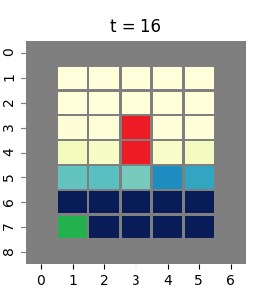
\includegraphics[scale=.5]{lowbb}}
	%\hfill
	\subfloat[$\beta = 5$\label{fig:simple-transitions}]{
		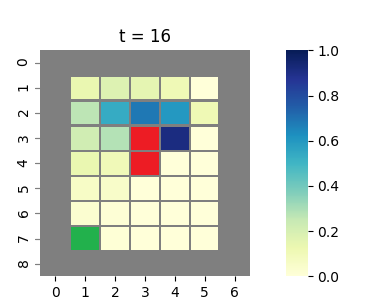
\includegraphics[scale=0.5]{highb}
	}
	\caption{Probability distribution of the agent after 16/25 timesteps. a) has a low $\beta$ which means information cost is low while b) has a high $\beta$ and hence high cost on information}
	\label{fig:expres}
\end{figure}

Figure \ref{fig:expres} shows the probability distributions of the agent at a specific time $t=16$. Clearly, in the case where $\beta=0.5$, the agent is able to go through the region where the moving obstacle operates. However, when we increase the cost of information, the agent moves around the static obstacles.


%%%%%%%%%%%%%%%%%%%%%%%%%%%%%%%%%%%%%%%%%%%%%%%%%%%%%%%%%%%%%%%%%%%%%%%%%%%%%%%%

\section{Conclusion and future work}
In this paper, we presented a formal way to integrate co-safe LTL constraints into a minimal-information MDP problem. This is the first step in analyzing temporal logic constraints in communication constrained problems. For future work, we aim to relax the co-safe requirement to allow more general classes of LTL formulas by analyzing the mean information cost over an infinite run. Furthermore, we aim to extend this work to a multiple coordinating agent formulation as this problem setting naturally lends itself to minimizing communication between agents who are trying to satisfy a joint specification. 



\bibliographystyle{IEEEtran}
\bibliography{main}

\appendices
\vspace{-0.15cm}
\section{Proof of Theorem 5.1} \label{sec:prf}

We first prove the following lemma.
\begin{lemma}
\label{lemcoding}
For each $T=1, 2, ...$, we have
\[
I(\bar{X}^{T} \rightarrow W^{T} || U^{T-1},\tilde{X}^{T}) \geq I(\bar{X}^{T} \rightarrow U^{T} || \tilde{X}^{T}).
\]
\end{lemma}
\begin{proof}
The result is established by the following chain of inequalities.
\begin{align*}
&  I(\bar{X}^T \rightarrow W^T || U^{T-1},\tilde{X}^T) - I(\bar{X}^T \rightarrow U^T || \tilde{X}^T)  \\
& = \sum_{t=0}^T I\left(\bar{X}^t;W_t|W^{t-1},U^{t-1},\tilde{X}^t \right) - I\left(\bar{X}^t;U_t|U^{t-1},\tilde{X}^t \right)\\
& \stackrel{\text{(a)}}{=} \sum_{t=0}^T I\left(\bar{X}^t;W_t,U_t|W^{t-1},U^{t-1},\tilde{X}^t \right) \\
& \hspace{10ex}- I\left(\bar{X}^t;U_t|U^{t-1},\tilde{X}^t \right)\\
& \stackrel{\text{(b)}}{=} \sum_{t=0}^T I\left(\bar{X}^t;W^t|U^{t},\tilde{X}^t \right) - I\left(\bar{X}^t;W^{t-1}|U^{t-1},\tilde{X}^t \right)\\
& \stackrel{\text{(c)}}{=} \sum_{t=0}^T I\left(\bar{X}^t;W^t|U^{t},\tilde{X}^t \right) - I\left(\bar{X}^{t-1};W^{t-1}|U^{t-1},\tilde{X}^t \right)\\
& \stackrel{\text{(d)}}{\geq} \sum_{t=0}^T I\left(\bar{X}^t;W^t|U^{t},\tilde{X}^t \right) - I\left(\bar{X}^{t-1};W^{t-1}|U^{t-1},\tilde{X}^{t-1} \right)\\
& \stackrel{\text{(e)}}{=} I\left(\bar{X}^T;W^T | U^T,\tilde{X}^T \right) \geq 0. 
\end{align*}
Equality (a) holds since
\begin{align*}
&I(\bar{X}^t; W_t, U_t|W^{t-1}, U^{t-1}, \tilde{X}^t)=\\
&I(\bar{X}^t; W_t|W^{t-1}, U^{t-1}, \tilde{X}^t)
+I(\bar{X}^t; U_t|W^t, U^{t-1}, \tilde{X}^t)
\end{align*}
and the second term is zero since $U_t$ is conditionally independent of $\bar{X}^t$ given $(W^t, U^{t-1})$. Equality (b) can be shown by applying the chain rule for mutual information in two different ways:
\begin{align*}
&I(\bar{X}^t; W^t, U_t|U^{t-1}, \tilde{X}^t) \\
&=I(\bar{X}^t; W^{t-1}|U^{t-1}, \tilde{X}^t)+I(\bar{X}^t; W_t, U_t| W^{t-1}, U^{t-1}, \tilde{X}^t) \\
&=I(\bar{X}^t; U_t|U^{t-1}, \tilde{X}^t)+I(\bar{X}^t;W^t|U^t, \tilde{X}^t).
\end{align*}
Equality (c) holds since
\begin{align*}
&I(\bar{X}^t; W^{t-1}|U^{t-1}, \tilde{X}^t)=\\
&I(\bar{X}^{t-1}; W^{t-1}|U^{t-1}, \tilde{X}^t)+I(\bar{X}_t; W^{t-1}|U^{t-1}, \tilde{X}^t, \bar{X}^{t-1})
\end{align*}
and the second term is zero. To see (d), apply the chain rule in two different ways:
\begin{align*}
&I(\bar{X}^{t-1}, \tilde{X}_t; W^{t-1}|U^{t-1},\tilde{X}^{t-1}) \\
&=I(\tilde{X}_t; W^{t-1}|U^{t-1}, \tilde{X}^{t-1})+I(\bar{X}^{t-1}; W^{t-1}|U^{t-1}, \tilde{X}^t) \\
&=I(\bar{X}^{t-1}; W^{t-1}|U^{t-1}, \tilde{X}^{t-1}) \\
&\hspace{5ex}+I(\tilde{X}_t;W^{t-1}|U^{t-1},\tilde{X}^{t-1}, \bar{X}^{t-1}).
\end{align*}
Since the last term is zero, we have 
\[
I(\bar{X}^{t-1}; W^{t-1}|U^{t-1}, \tilde{X}^{t-1}) \geq I(\bar{X}^{t-1}; W^{t-1}|U^{t-1}, \tilde{X}^t).
\]
Finally, (e) is due to the telescopic cancellation.
\end{proof}

Theorem~\ref{theorate} can now be shown as
\begin{align*}
R&=\sum_{t=0}^{T-1} R_t \\
&\stackrel{\text{(a)}}{\geq} \sum\nolimits_{t=0}^{T-1} H(W_t) \\
&\stackrel{\text{(b)}}{\geq} \sum\nolimits_{t=0}^{T-1} H(W_t|W^{t-1}, U^{t-1}, \tilde{X}^t) \\
&\stackrel{\text{(c)}}{\geq} \sum\nolimits_{t=0}^{T-1} H(W_t|W^{t-1}, U^{t-1}, \tilde{X}^t) \\
&\hspace{10ex}-H(W_t|\bar{X}^t, W^{t-1}, U^{t-1}, \tilde{X}^t) \\
&=\sum\nolimits_{t=0}^{T-1} I(\bar{X}^t; W_t|W^{t-1}, U^{t-1}, \tilde{X}^t) \\
&=I(\bar{X}^{T-1}\rightarrow W^{T-1}\| U^{T-2}, \tilde{X}^{T-1}) \\
&\stackrel{\text{(d)}}{\geq} I(\bar{X}^{T-1}\rightarrow U^{T-1}\| \tilde{X}^{T-1})
\end{align*}
Inequality (a) is a standard result - Theorem 2.6.4 in \cite{cover2012elements}. Inequality (b) holds since conditioning does not increase entropy, and (c) is because entropy is non-negative. Finally, (d) is due to Lemma~\ref{lemcoding}.



\end{document}
